\documentclass{article}
\usepackage[margin=0.25in,landscape,a3paper]{geometry}
\usepackage{lmodern}
\usepackage{tikz}
\usepackage{xcolor}
\pagestyle{empty}
\usetikzlibrary{shapes,arrows,positioning,calc,fit,backgrounds,decorations.pathreplacing}

\begin{document}
\begin{center}
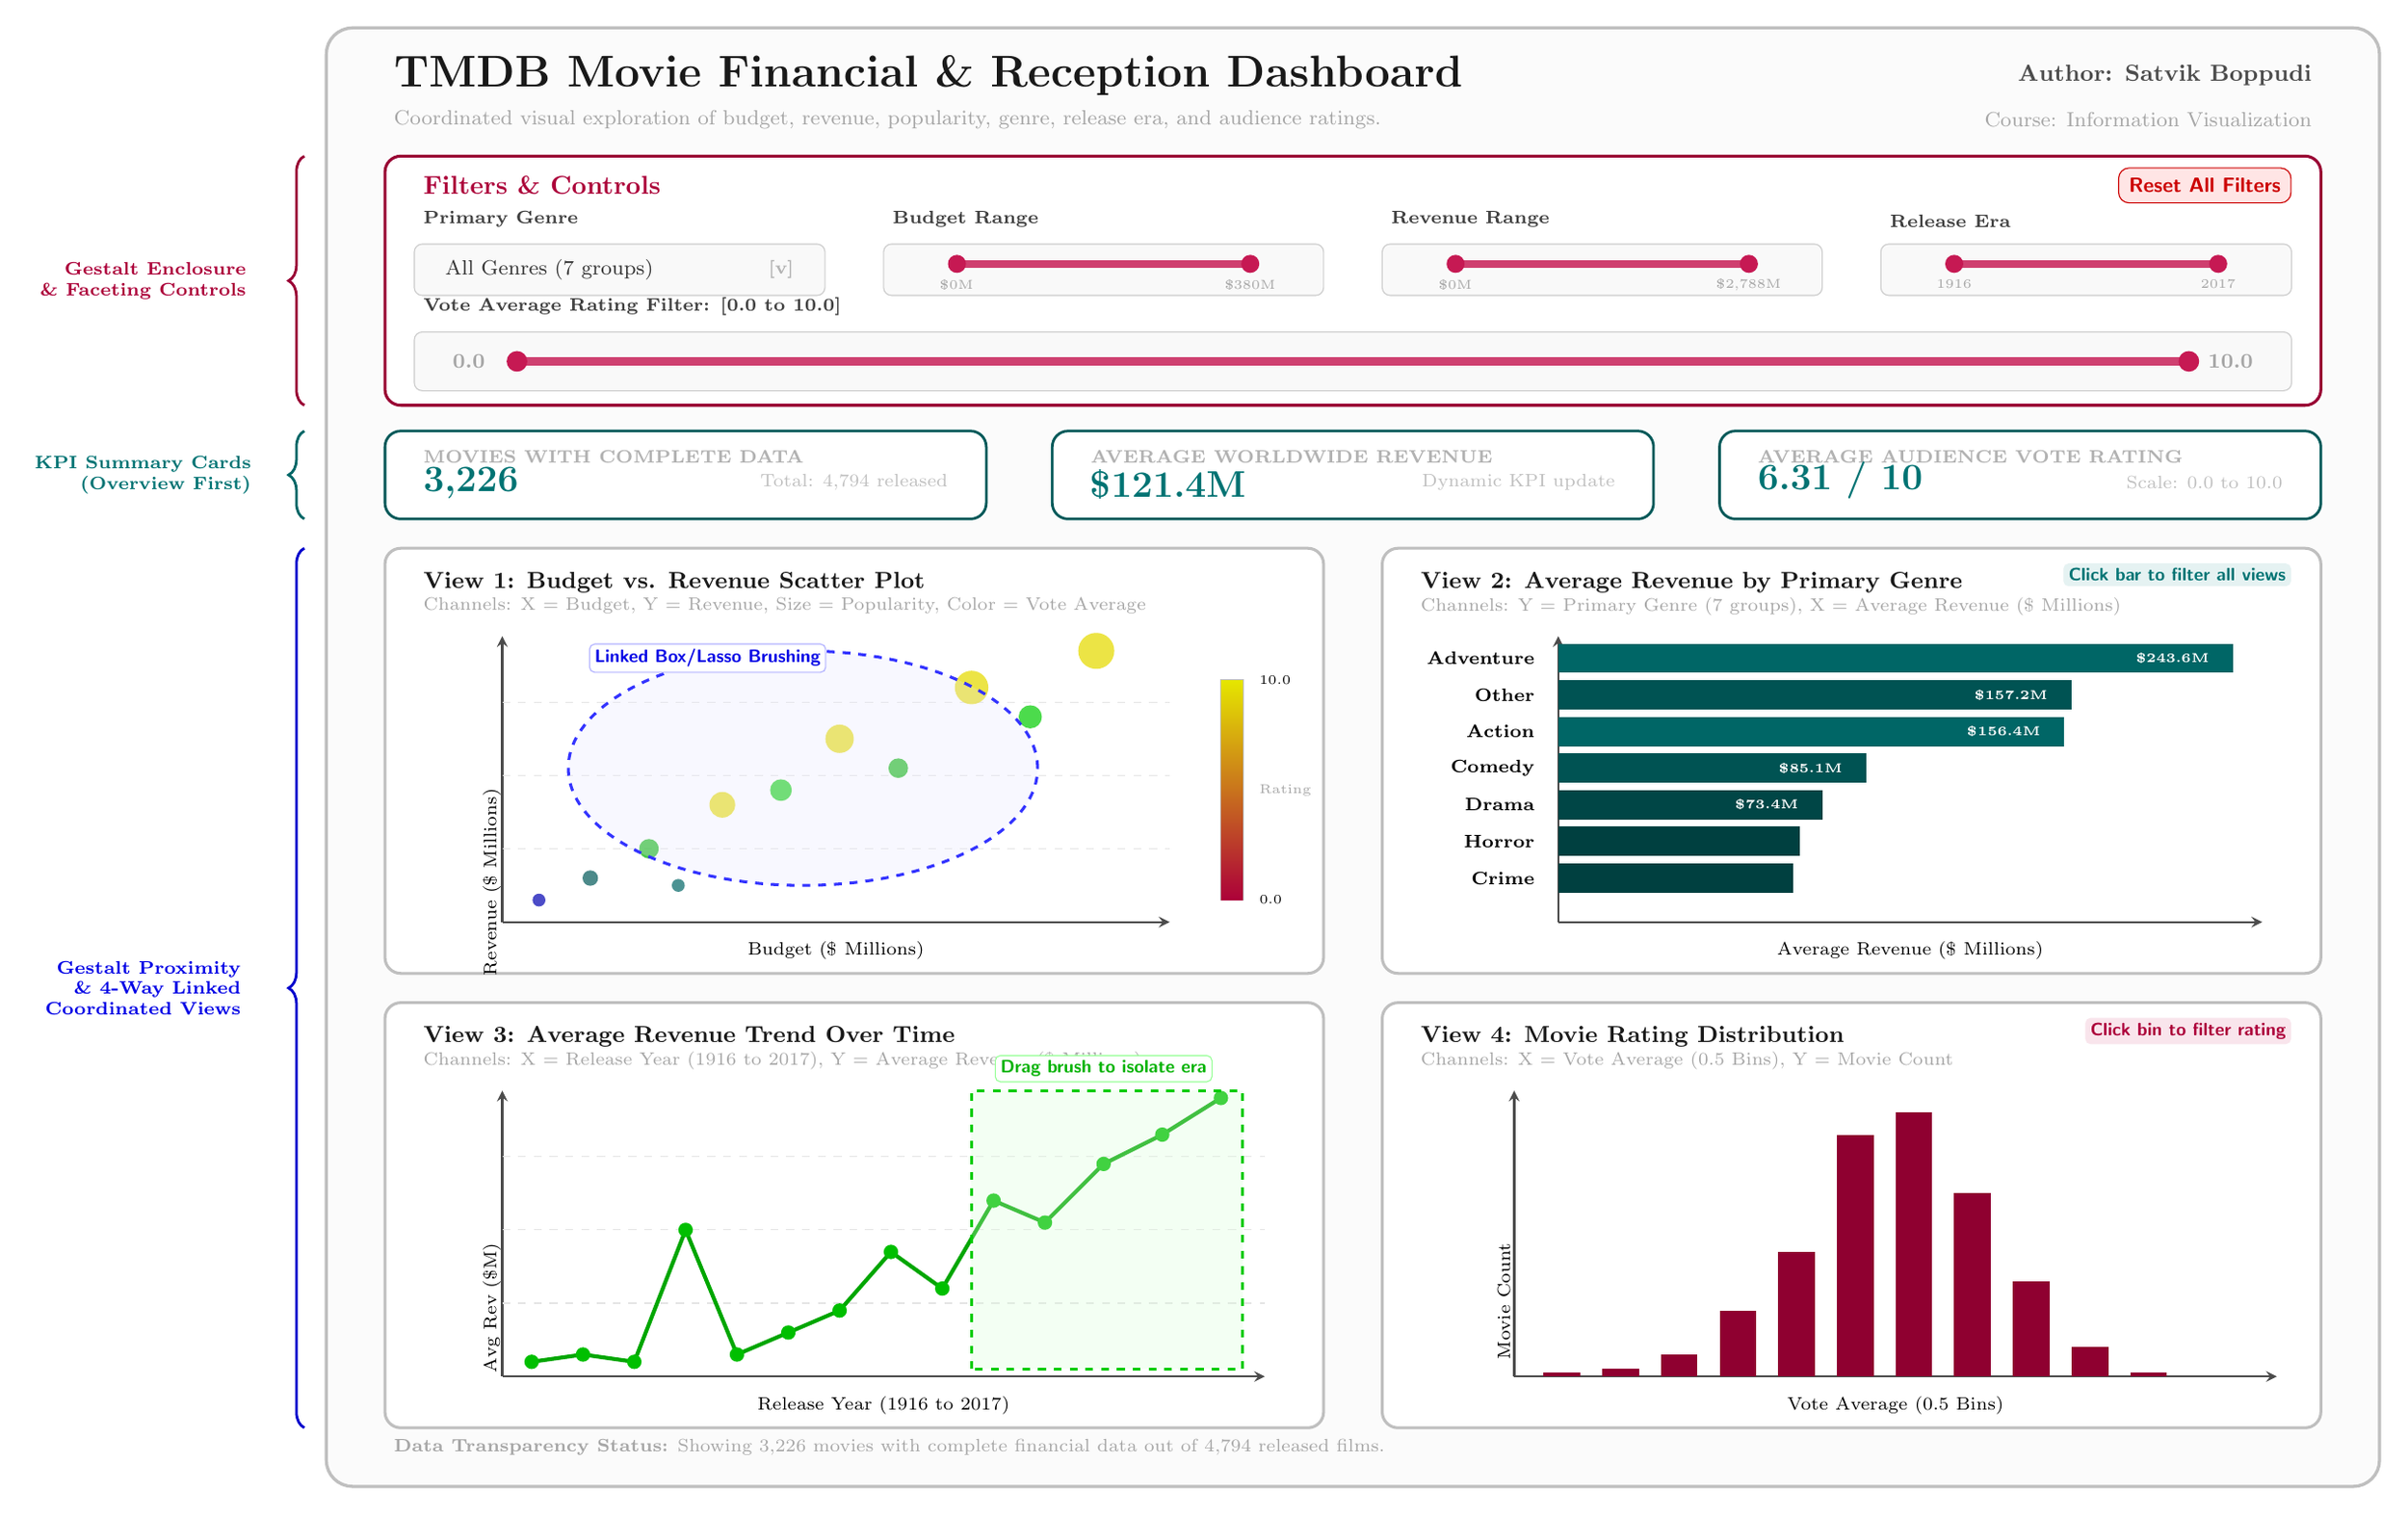
\begin{tikzpicture}[
    font=\sffamily,
    scale=0.98, every node/.style={transform shape},
    canvas/.style={draw=black!25, fill=gray!3, rounded corners=10pt, line width=1.2pt},
    filterbox/.style={draw=purple!80!black, fill=white, rounded corners=6pt, line width=1.1pt},
    kpicard/.style={draw=teal!70!black, fill=white, rounded corners=6pt, line width=1.0pt},
    chartcard/.style={draw=gray!50, fill=white, rounded corners=6pt, line width=1.1pt},
    button/.style={draw=red!80!black, fill=red!10, rounded corners=4pt, font=\sffamily\bfseries\footnotesize, text=red!80!black, inner sep=4pt},
    axis/.style={->, >=stealth, line width=0.8pt, draw=black!70},
    callout/.style={font=\sffamily\bfseries\scriptsize, align=center}
]

% ==============================================================================
% 0. MAIN DASHBOARD CANVAS CONTAINER
% ==============================================================================
\draw[canvas] (0, 2.7) rectangle (28, -17.2);

% ==============================================================================
% 1. HEADER
% ==============================================================================
\node[anchor=west, font=\LARGE\bfseries, text=black!90] at (0.8, 2.05) {TMDB Movie Financial \& Reception Dashboard};
\node[anchor=west, font=\footnotesize, text=gray!70] at (0.8, 1.45) {Coordinated visual exploration of budget, revenue, popularity, genre, release era, and audience ratings.};

\node[anchor=east, font=\small\bfseries, text=black!70] at (27.2, 2.05) {Author: Satvik Boppudi};
\node[anchor=east, font=\footnotesize, text=gray!70] at (27.2, 1.45) {Course: Information Visualization};

% ==============================================================================
% 2. GLOBAL FILTERS PANEL
% ==============================================================================
\draw[filterbox] (0.8, 0.95) rectangle (27.2, -2.45);

% Panel Header & Reset Button
\node[anchor=west, font=\bfseries\normalsize, text=purple!90!black] at (1.2, 0.55) {Filters \& Controls};
\node[button, anchor=east] at (26.8, 0.55) {Reset All Filters};

% Filter Row 1 (4 Columns)
% Col 1: Genre Dropdown (X: 1.2 to 6.8)
\node[anchor=south west, font=\scriptsize\bfseries, text=black!75] at (1.2, -0.15) {Primary Genre};
\draw[draw=gray!40, fill=gray!5, rounded corners=3pt] (1.2, -0.25) rectangle (6.8, -0.95);
\node[anchor=west, font=\footnotesize, text=black!80] at (1.5, -0.6) {All Genres (7 groups)};
\node[anchor=east, font=\scriptsize\bfseries, text=gray!60] at (6.5, -0.6) {[v]};

% Col 2: Budget Slider (X: 7.6 to 13.6)
\node[anchor=south west, font=\scriptsize\bfseries, text=black!75] at (7.6, -0.15) {Budget Range};
\draw[draw=gray!40, fill=gray!5, rounded corners=3pt] (7.6, -0.25) rectangle (13.6, -0.95);
\draw[line width=3pt, gray!30] (8.6, -0.52) -- (12.6, -0.52);
\draw[line width=3pt, purple!75] (8.6, -0.52) -- (12.6, -0.52);
\fill[purple!90] (8.6, -0.52) circle (3.5pt);
\fill[purple!90] (12.6, -0.52) circle (3.5pt);
\node[font=\tiny, text=gray!70] at (8.6, -0.8) {\$0M};
\node[font=\tiny, text=gray!70] at (12.6, -0.8) {\$380M};

% Col 3: Revenue Slider (X: 14.4 to 20.4)
\node[anchor=south west, font=\scriptsize\bfseries, text=black!75] at (14.4, -0.15) {Revenue Range};
\draw[draw=gray!40, fill=gray!5, rounded corners=3pt] (14.4, -0.25) rectangle (20.4, -0.95);
\draw[line width=3pt, gray!30] (15.4, -0.52) -- (19.4, -0.52);
\draw[line width=3pt, purple!75] (15.4, -0.52) -- (19.4, -0.52);
\fill[purple!90] (15.4, -0.52) circle (3.5pt);
\fill[purple!90] (19.4, -0.52) circle (3.5pt);
\node[font=\tiny, text=gray!70] at (15.4, -0.8) {\$0M};
\node[font=\tiny, text=gray!70] at (19.4, -0.8) {\$2,788M};

% Col 4: Release Year Slider (X: 21.2 to 26.8)
\node[anchor=south west, font=\scriptsize\bfseries, text=black!75] at (21.2, -0.15) {Release Era};
\draw[draw=gray!40, fill=gray!5, rounded corners=3pt] (21.2, -0.25) rectangle (26.8, -0.95);
\draw[line width=3pt, gray!30] (22.2, -0.52) -- (25.8, -0.52);
\draw[line width=3pt, purple!75] (22.2, -0.52) -- (25.8, -0.52);
\fill[purple!90] (22.2, -0.52) circle (3.5pt);
\fill[purple!90] (25.8, -0.52) circle (3.5pt);
\node[font=\tiny, text=gray!70] at (22.2, -0.8) {1916};
\node[font=\tiny, text=gray!70] at (25.8, -0.8) {2017};

% Filter Row 2: Vote Average Slider (X: 1.2 to 26.8)
\node[anchor=south west, font=\scriptsize\bfseries, text=black!75] at (1.2, -1.35) {Vote Average Rating Filter: [0.0 to 10.0]};
\draw[draw=gray!40, fill=gray!5, rounded corners=3pt] (1.2, -1.45) rectangle (26.8, -2.25);
\node[anchor=west, font=\footnotesize\bfseries, text=gray!70] at (1.6, -1.85) {0.0};
\draw[line width=3.5pt, gray!30] (2.6, -1.85) -- (25.4, -1.85);
\draw[line width=3.5pt, purple!75] (2.6, -1.85) -- (25.4, -1.85);
\fill[purple!90] (2.6, -1.85) circle (4pt);
\fill[purple!90] (25.4, -1.85) circle (4pt);
\node[anchor=east, font=\footnotesize\bfseries, text=gray!70] at (26.4, -1.85) {10.0};

% ==============================================================================
% 3. KPI SUMMARY ROW
% ==============================================================================
% KPI 1 (X: 0.8 to 9.0)
\draw[kpicard] (0.8, -2.8) rectangle (9.0, -4.0);
\node[anchor=north west, font=\scriptsize\bfseries, text=gray!60] at (1.2, -2.95) {MOVIES WITH COMPLETE DATA};
\node[anchor=south west, font=\Large\bfseries, text=teal!90!black] at (1.2, -3.85) {3,226};
\node[anchor=east, font=\scriptsize, text=gray!50] at (8.6, -3.5) {Total: 4,794 released};

% KPI 2 (X: 9.9 to 18.1)
\draw[kpicard] (9.9, -2.8) rectangle (18.1, -4.0);
\node[anchor=north west, font=\scriptsize\bfseries, text=gray!60] at (10.3, -2.95) {AVERAGE WORLDWIDE REVENUE};
\node[anchor=south west, font=\Large\bfseries, text=teal!90!black] at (10.3, -3.85) {\$121.4M};
\node[anchor=east, font=\scriptsize, text=gray!50] at (17.7, -3.5) {Dynamic KPI update};

% KPI 3 (X: 19.0 to 27.2)
\draw[kpicard] (19.0, -2.8) rectangle (27.2, -4.0);
\node[anchor=north west, font=\scriptsize\bfseries, text=gray!60] at (19.4, -2.95) {AVERAGE AUDIENCE VOTE RATING};
\node[anchor=south west, font=\Large\bfseries, text=teal!90!black] at (19.4, -3.85) {6.31 / 10};
\node[anchor=east, font=\scriptsize, text=gray!50] at (26.8, -3.5) {Scale: 0.0 to 10.0};

% ==============================================================================
% 4. COORDINATED 2x2 ANALYTICAL GRID
% ==============================================================================

% ------------------------------------------------------------------------------
% VIEW 1: SCATTER PLOT (Top Left: X: 0.8 to 13.6, Y: -4.4 to -10.2)
% ------------------------------------------------------------------------------
\draw[chartcard] (0.8, -4.4) rectangle (13.6, -10.2);
\node[anchor=north west, font=\small\bfseries, text=black!90] at (1.2, -4.6) {View 1: Budget vs. Revenue Scatter Plot};
\node[anchor=north west, font=\scriptsize, text=gray!70] at (1.2, -4.95) {Channels: X = Budget, Y = Revenue, Size = Popularity, Color = Vote Average};

% Scatter Axes
\draw[axis] (2.4, -9.5) -- (11.5, -9.5) node[midway, below=4pt, font=\scriptsize] {Budget (\$ Millions)};
\draw[axis] (2.4, -9.5) -- (2.4, -5.6) node[midway, left=4pt, font=\scriptsize, rotate=90] {Revenue (\$ Millions)};

% Grid lines
\draw[dashed, gray!20] (2.4, -8.5) -- (11.5, -8.5);
\draw[dashed, gray!20] (2.4, -7.5) -- (11.5, -7.5);
\draw[dashed, gray!20] (2.4, -6.5) -- (11.5, -6.5);

% Plotted Scatter Points
\fill[blue!70!black, opacity=0.7] (2.9, -9.2) circle (2.5pt);
\fill[teal!70!black, opacity=0.7] (3.6, -8.9) circle (3.0pt);
\fill[green!70!black, opacity=0.7] (4.4, -8.5) circle (3.8pt);
\fill[teal!80!black, opacity=0.7] (4.8, -9.0) circle (2.5pt);
\fill[yellow!90!black, opacity=0.8] (5.4, -7.9) circle (5.0pt);
\fill[green!80!black, opacity=0.7] (6.2, -7.7) circle (4.2pt);
\fill[yellow!90!black, opacity=0.8] (7.0, -7.0) circle (5.5pt);
\fill[green!70!black, opacity=0.7] (7.8, -7.4) circle (3.8pt);
\fill[yellow!90!black, opacity=0.8] (8.8, -6.3) circle (6.5pt);
\fill[green!80!black, opacity=0.7] (9.6, -6.7) circle (4.5pt);
\fill[yellow!90!black, opacity=0.8] (10.5, -5.8) circle (7.0pt);

% Linked Lasso/Box Selection
\draw[draw=blue!80, dashed, line width=1.1pt, fill=blue!10, fill opacity=0.25] (6.5, -7.4) ellipse (3.2cm and 1.6cm);
\node[callout, text=blue!90!black, fill=white, inner sep=2pt, rounded corners=2pt, draw=blue!30] at (5.2, -5.9) {Linked Box/Lasso Brushing};

% Viridis Color Legend Bar
\draw[draw=gray!50, line width=0.5pt] (12.2, -6.2) rectangle (12.5, -9.2);
\shade[top color=yellow!90!black, bottom color=purple!90!black] (12.2, -6.2) rectangle (12.5, -9.2);
\node[font=\tiny, anchor=west] at (12.6, -6.2) {10.0};
\node[font=\tiny, anchor=west, text=gray!70] at (12.6, -7.7) {Rating};
\node[font=\tiny, anchor=west] at (12.6, -9.2) {0.0};

% ------------------------------------------------------------------------------
% VIEW 2: GENRE BAR CHART (Top Right: X: 14.4 to 27.2, Y: -4.4 to -10.2)
% ------------------------------------------------------------------------------
\draw[chartcard] (14.4, -4.4) rectangle (27.2, -10.2);
\node[anchor=north west, font=\small\bfseries, text=black!90] at (14.8, -4.6) {View 2: Average Revenue by Primary Genre};
\node[anchor=north west, font=\scriptsize, text=gray!70] at (14.8, -4.95) {Channels: Y = Primary Genre (7 groups), X = Average Revenue (\$ Millions)};

\node[callout, text=teal!90!black, fill=teal!10, inner sep=2pt, rounded corners=2pt, anchor=north east] at (26.8, -4.6) {Click bar to filter all views};

% Axes
\draw[axis] (16.8, -9.5) -- (26.4, -9.5) node[midway, below=4pt, font=\scriptsize] {Average Revenue (\$ Millions)};
\draw[axis] (16.8, -9.5) -- (16.8, -5.6);

% Horizontal Bars
\node[font=\scriptsize\bfseries, anchor=east] at (16.6, -5.9) {Adventure};
\fill[teal!80!black] (16.8, -6.1) rectangle (26.0, -5.7);
\node[font=\tiny\bfseries, text=white, anchor=east] at (25.8, -5.9) {\$243.6M};

\node[font=\scriptsize\bfseries, anchor=east] at (16.6, -6.4) {Other};
\fill[teal!65!black] (16.8, -6.6) rectangle (23.8, -6.2);
\node[font=\tiny\bfseries, text=white, anchor=east] at (23.6, -6.4) {\$157.2M};

\node[font=\scriptsize\bfseries, anchor=east] at (16.6, -6.9) {Action};
\fill[teal!80!black] (16.8, -7.1) rectangle (23.7, -6.7);
\node[font=\tiny\bfseries, text=white, anchor=east] at (23.5, -6.9) {\$156.4M};

\node[font=\scriptsize\bfseries, anchor=east] at (16.6, -7.4) {Comedy};
\fill[teal!65!black] (16.8, -7.6) rectangle (21.0, -7.2);
\node[font=\tiny\bfseries, text=white, anchor=east] at (20.8, -7.4) {\$85.1M};

\node[font=\scriptsize\bfseries, anchor=east] at (16.6, -7.9) {Drama};
\fill[teal!55!black] (16.8, -8.1) rectangle (20.4, -7.7);
\node[font=\tiny\bfseries, text=white, anchor=east] at (20.2, -7.9) {\$73.4M};

\node[font=\scriptsize\bfseries, anchor=east] at (16.6, -8.4) {Horror};
\fill[teal!50!black] (16.8, -8.6) rectangle (20.1, -8.2);

\node[font=\scriptsize\bfseries, anchor=east] at (16.6, -8.9) {Crime};
\fill[teal!50!black] (16.8, -9.1) rectangle (20.0, -8.7);

% ------------------------------------------------------------------------------
% VIEW 3: TIMELINE CHART (Bottom Left: X: 0.8 to 13.6, Y: -10.6 to -16.4)
% ------------------------------------------------------------------------------
\draw[chartcard] (0.8, -10.6) rectangle (13.6, -16.4);
\node[anchor=north west, font=\small\bfseries, text=black!90] at (1.2, -10.8) {View 3: Average Revenue Trend Over Time};
\node[anchor=north west, font=\scriptsize, text=gray!70] at (1.2, -11.15) {Channels: X = Release Year (1916 to 2017), Y = Average Revenue (\$ Millions)};

% Axes
\draw[axis] (2.4, -15.7) -- (12.8, -15.7) node[midway, below=4pt, font=\scriptsize] {Release Year (1916 to 2017)};
\draw[axis] (2.4, -15.7) -- (2.4, -11.8) node[midway, left=4pt, font=\scriptsize, rotate=90] {Avg Rev (\$M)};

% Grid lines
\draw[dashed, gray!20] (2.4, -14.7) -- (12.8, -14.7);
\draw[dashed, gray!20] (2.4, -13.7) -- (12.8, -13.7);
\draw[dashed, gray!20] (2.4, -12.7) -- (12.8, -12.7);

% Trend Line
\draw[line width=1.5pt, green!65!black] 
    (2.8, -15.5) -- (3.5, -15.4) -- (4.2, -15.5) -- (4.9, -13.7) -- 
    (5.6, -15.4) -- (6.3, -15.1) -- (7.0, -14.8) -- (7.7, -14.0) -- 
    (8.4, -14.5) -- (9.1, -13.3) -- (9.8, -13.6) -- (10.6, -12.8) -- 
    (11.4, -12.4) -- (12.2, -11.9);

\foreach \pt in {(2.8, -15.5), (3.5, -15.4), (4.2, -15.5), (4.9, -13.7), 
                 (5.6, -15.4), (6.3, -15.1), (7.0, -14.8), (7.7, -14.0), 
                 (8.4, -14.5), (9.1, -13.3), (9.8, -13.6), (10.6, -12.8), 
                 (11.4, -12.4), (12.2, -11.9)} {
    \fill[green!75!black] \pt circle (2.8pt);
}

% Era Selection Box
\draw[draw=green!80!black, dashed, line width=1.1pt, fill=green!15, fill opacity=0.3] (8.8, -15.6) rectangle (12.5, -11.8);
\node[callout, text=green!70!black, fill=white, inner sep=2pt, rounded corners=2pt, draw=green!40] at (10.6, -11.5) {Drag brush to isolate era};

% ------------------------------------------------------------------------------
% VIEW 4: RATING HISTOGRAM (Bottom Right: X: 14.4 to 27.2, Y: -10.6 to -16.4)
% ------------------------------------------------------------------------------
\draw[chartcard] (14.4, -10.6) rectangle (27.2, -16.4);
\node[anchor=north west, font=\small\bfseries, text=black!90] at (14.8, -10.8) {View 4: Movie Rating Distribution};
\node[anchor=north west, font=\scriptsize, text=gray!70] at (14.8, -11.15) {Channels: X = Vote Average (0.5 Bins), Y = Movie Count};

\node[callout, text=purple!90!black, fill=purple!10, inner sep=2pt, rounded corners=2pt, anchor=north east] at (26.8, -10.8) {Click bin to filter rating};

% Axes
\draw[axis] (16.2, -15.7) -- (26.6, -15.7) node[midway, below=4pt, font=\scriptsize] {Vote Average (0.5 Bins)};
\draw[axis] (16.2, -15.7) -- (16.2, -11.8) node[midway, left=4pt, font=\scriptsize, rotate=90] {Movie Count};

% Histogram Bars
\fill[purple!75!black] (16.6, -15.7) rectangle (17.1, -15.65);
\fill[purple!75!black] (17.4, -15.7) rectangle (17.9, -15.6);
\fill[purple!75!black] (18.2, -15.7) rectangle (18.7, -15.4);
\fill[purple!75!black] (19.0, -15.7) rectangle (19.5, -14.8);
\fill[purple!75!black] (19.8, -15.7) rectangle (20.3, -14.0);
\fill[purple!75!black] (20.6, -15.7) rectangle (21.1, -12.4);
\fill[purple!75!black] (21.4, -15.7) rectangle (21.9, -12.1);
\fill[purple!75!black] (22.2, -15.7) rectangle (22.7, -13.2);
\fill[purple!75!black] (23.0, -15.7) rectangle (23.5, -14.4);
\fill[purple!75!black] (23.8, -15.7) rectangle (24.3, -15.3);
\fill[purple!75!black] (24.6, -15.7) rectangle (25.1, -15.65);

% ==============================================================================
% 5. SIDE GESTALT ANNOTATIONS
% ==============================================================================
\draw[decorate, decoration={brace, amplitude=6pt, mirror}, line width=1.0pt, draw=purple!80!black]
    (-0.3, 0.95) -- (-0.3, -2.45) node[midway, xshift=-2.2cm, font=\scriptsize\bfseries, text=purple!90!black, align=right] {Gestalt Enclosure\\\& Faceting Controls};

\draw[decorate, decoration={brace, amplitude=6pt, mirror}, line width=1.0pt, draw=teal!80!black]
    (-0.3, -2.8) -- (-0.3, -4.0) node[midway, xshift=-2.2cm, font=\scriptsize\bfseries, text=teal!90!black, align=right] {KPI Summary Cards\\(Overview First)};

\draw[decorate, decoration={brace, amplitude=6pt, mirror}, line width=1.0pt, draw=blue!80!black]
    (-0.3, -4.4) -- (-0.3, -16.4) node[midway, xshift=-2.2cm, font=\scriptsize\bfseries, text=blue!90!black, align=right] {Gestalt Proximity\\\& 4-Way Linked\\Coordinated Views};

% Bottom Status Bar
\node[anchor=south west, font=\scriptsize, text=gray!70] at (0.8, -16.9) {\textbf{Data Transparency Status:} Showing 3,226 movies with complete financial data out of 4,794 released films.};

\end{tikzpicture}
\end{center}
\end{document}
